\begin{center}
{\large\bfseries ПРИЛОЖЕНИЕ К СТАТЬЕ «СВОЕВРЕМЕННОЕ НАЧАЛО ПАКЕТНОГО ОБСЛУЖИВАНИЯ ПРИ НЕТЕРПЕНИИ ЗАЯВОК»}

Р.С.~Хабаров, В.А.~Лохвицкий
\end{center}

Здесь приведены подробности марковской конструкции, доказательство локальной оценки погрешности и вспомогательные численные результаты. Обозначения согласованы с основным текстом: $a$ --- порог запуска, $b$ --- максимальный размер пакета, $\lambda$ --- интенсивность входящего потока, $\gamma$ --- интенсивность ухода ожидающей заявки. Закон времени обслуживания пакета размера $i$ задаётся вероятностным фазовым представлением $(\beta_i,T_i)$ с поглощением с вероятностью единица.

Событие $S$ означает начало обслуживания помеченной заявки, $p_S=P(S)$, $p_A$ --- вероятность её ухода, $W$ --- время ожидания на событии $S$. Для срока $D$ обозначены $S(D)=P(S,W\leq D)$ и $L(D)=P(S,W>D)$; условная ДФР равна $\overline F_S(D)=L(D)/p_S$ при $p_S>0$. Полное время пребывания до завершения обслуживания обозначено $V$.


\section*{А. Конструкция процесса ожидания}

При занятом канале состояние системы задаётся тройкой $(i,\varphi,j)$, где $i$ --- размер обслуживаемого пакета, $\varphi$ --- текущая фаза обслуживания, $j$ --- число заявок в очереди. Состояние простоя обозначим $I_j$, $0\leq j<a$. Поступление заявки увеличивает $j$ на единицу, а уход из очереди уменьшает его на единицу с суммарной интенсивностью $j\gamma$. Переходы между фазами задаются матрицей $T_i$; интенсивность завершения обслуживания из фазы $\varphi$ равна соответствующей компоненте вектора $\nu_i=-T_i\mathbf1$, где $\mathbf1$ --- столбец единиц. После завершения обслуживания при $j\geq a$ формируется пакет размера $m=\min(b,j)$, начальная фаза выбирается согласно распределению $\beta_m$, а в очереди остаются $j-m$ заявок. При $j<a$ система переходит в состояние $I_j$. Поступление заявки в состоянии $I_{a-1}$ приводит к началу обслуживания пакета размера $a$.

\begin{figure}[htbp]\centering
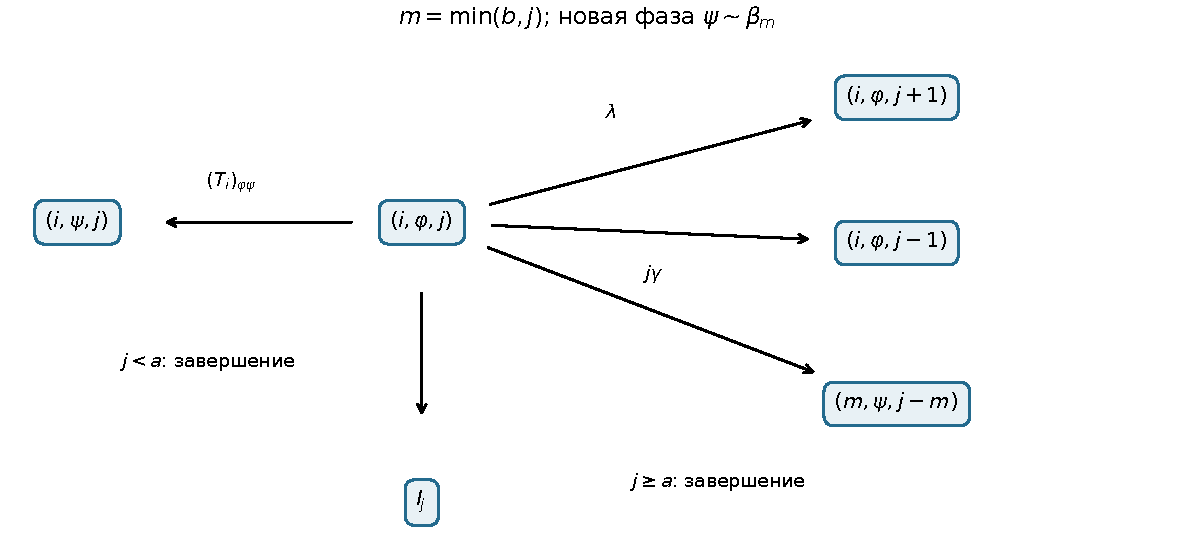
\includegraphics[width=\linewidth]{../figures/revision_queue.pdf}
\caption{Переходы из состояния с занятым каналом. После завершения обслуживания в следующий пакет включаются $m=\min(b,j)$ заявок. Интенсивности соответствующих переходов равны $\nu_{i,\varphi}\beta_{m,\psi}$, а при переходе в простой --- $\nu_{i,\varphi}$.}\label{fig:queue}
\end{figure}

Согласно принципу PASTA (Poisson Arrivals See Time Averages), распределение состояний, наблюдаемых поступающей заявкой, совпадает со стационарным распределением $\pi$. Вероятность немедленного начала обслуживания равна $p_0=\pi(I_{a-1})$: поступившая заявка застаёт свободный канал и $a-1$ ожидающих заявок, дополняя пакет до порога запуска. Среди заявок, начавших обслуживание, доля заявок с нулевым ожиданием равна $P(W=0\mid S)=p_0/p_S$. Поэтому условная функция распределения времени ожидания имеет в нуле скачок этой величины. Точку, в которой сосредоточена положительная вероятность, называют атомом распределения; здесь это атом в нуле.

Остальные стационарные вероятности задают начальное распределение процесса ожидания. Для численного расчёта $\pi$ используется приближение $\pi_N$, получаемое из системы $\pi_N Q_N=0$, $\pi_N\mathbf1=1$. Генератор $Q_N$ строится на состояниях с $j\leq N$ с исключением переходов, соответствующих поступлению заявки при $j=N$.

Проследим за заявкой, не начавшей обслуживание немедленно, от её поступления до начала обслуживания или ухода из очереди. Через $R$ и $K$ обозначим числа заявок, ожидающих соответственно перед ней и позади неё. Если поступившая заявка застала $j$ ожидающих, начальные значения равны $R=j$, $K=0$. Состояние включает также режим канала, а при занятом канале --- размер текущего пакета и фазу обслуживания. Уже обслуживаемые заявки в $R$ и $K$ не входят. Наряду с переходами между фазами и уходом помеченной заявки с интенсивностью $\gamma$ учитываются переходы
\begin{equation}
 R\longrightarrow R-1\quad(R\gamma),\qquad
 K\longrightarrow K+1\quad(\lambda),\qquad
 K\longrightarrow K-1\quad(K\gamma),
\end{equation}
Интенсивности указаны в скобках. Переходы при завершении обслуживания пакета показаны на рисунке~\ref{fig:tagged}.

\begin{figure}[htbp]\centering
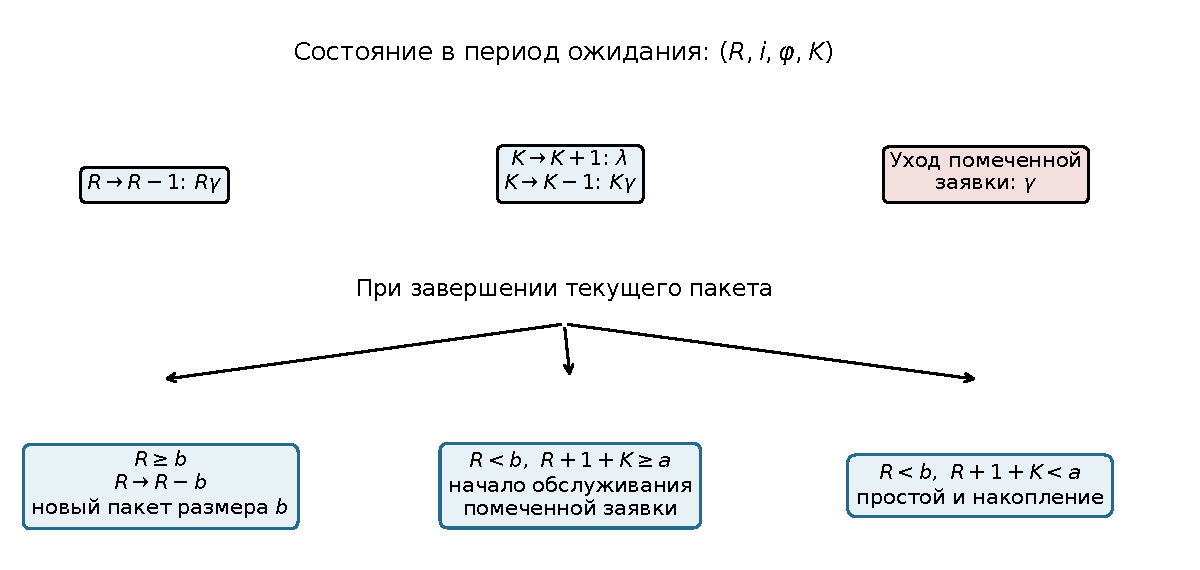
\includegraphics[width=\linewidth]{../figures/revision_tagged.pdf}
\caption{Процесс ожидания помеченной заявки: учёт числа заявок перед ней и позади неё. При простое продолжаются поступления и уходы заявок; обслуживание начинается при достижении порога запуска.}\label{fig:tagged}
\end{figure}

Если сформированный после поступления помеченной заявки пакет не включает её, его размер равен $b$. Действительно, при меньшем размере пакета все ожидающие заявки, в том числе помеченная, должны были бы войти в него в соответствии с дисциплиной FIFO. Следовательно, произвольный размер $i$ имеет только пакет, обслуживаемый в момент поступления помеченной заявки. При $R\geq b$ завершение текущего обслуживания приводит к началу обслуживания полного пакета: число $R$ уменьшается на $b$, а начальная фаза выбирается заново согласно $\beta_b$. При $R<b$ помеченная заявка поступает на обслуживание тогда и только тогда, когда $R+1+K\geq a$. В противном случае канал простаивает до накопления необходимого числа заявок.

Для численного расчёта ограничим число заявок позади условием $K\leq C$ и выберем конечное множество начальных состояний. Обозначим через $T$ подгенератор на состояниях продолжающегося ожидания, через $s$ --- столбец интенсивностей начала обслуживания, через $\alpha$ --- начальный вектор весов этих состояний, полученный из стационарного распределения. Вероятность немедленного начала обслуживания $p_0$ учитывается отдельно; вектор $\alpha$ не нормируется к единице. Два вида поглощения --- начало обслуживания и уход --- задают равенство $T\mathbf1+s+\gamma\mathbf1=0$. По стандартным формулам для цепи Маркова с поглощением получаем
\begin{align}
 h&=(-T)^{-1}s,& p_S&=p_0+\alpha h,\\
 L(D)&=\alpha e^{TD}h,& p_A&=\gamma\alpha(-T)^{-1}\mathbf1,\label{eq:ph}\\
 E[W^n\mid S]&=\frac{n!\alpha(-T)^{-n-1}s}{p_S},&
 S(D)&=p_S-L(D).
\end{align}
Формула для моментов справедлива при $n\geq1$. В частности, $\overline F_S(0)=1-p_0/p_S$. Эти соотношения точны для конечной цепи и дают приближение для исходной системы с неограниченной очередью. Если исключены начальные состояния суммарной вероятности $\delta$, рассчитанные вероятности удовлетворяют равенству $p_S+p_A=1-\delta$; исключённая вероятность учитывается отдельно от вероятностей исходов.

\section*{Б. Локальная оценка погрешности}

При $a>1$ и $\gamma>0$ число $K$ определяет как возможность накопления пакета, так и интенсивность ухода заявок позади помеченной. Для конечного расчёта переходы из $K=C$ в $K=C+1$ исключаются. Погрешность такого усечения оценивается через вероятность достижения границы до истечения времени терпения помеченной заявки. При $a=1$ число $K$ не влияет на её ожидание и исключается из описания состояния. При $\gamma=0$ оно не уменьшается, поэтому значения $K\geq a-1$ можно объединить в одно состояние без погрешности.

\noindent\textbf{Утверждение.}
Пусть $a>1$, $\gamma>0$. Вспомогательный процесс $K(t)$ описывается схемой размножения и гибели с интенсивностями $\lambda$ и $k\gamma$, $K(0)=0$. Обозначим через $H_C$ момент первого перехода $C\to C+1$, а через $A\sim\operatorname{Exp}(\gamma)$ --- независимое время терпения помеченной заявки. Рассмотрим усечённый процесс, в котором исключены переходы из $C$ в $C+1$, где $C\geq a-1$. При одинаковом начальном состоянии абсолютная погрешность вероятности любого события, определяемого уходом или временем начала обслуживания помеченной заявки, не превосходит
\begin{equation}\label{eq:bound}
 B_0(C)=P(H_C<A)=e_0^{\mathsf T}M_C^{-1}\lambda e_C,
\end{equation}
где $e_k$ --- единичный вектор с ненулевой компонентой на месте $k$, а $M_C$ --- трёхдиагональная матрица размера $C+1$ с элементами
\begin{equation}
 (M_C)_{kk}=\lambda+(k+1)\gamma,\quad
 (M_C)_{k,k+1}=-\lambda,\quad (M_C)_{k,k-1}=-k\gamma.
\end{equation}
Для ненормированных моментов $E[W^n\mathbf1_S]$, где $\mathbf1_S$ --- индикатор события $S$, соответствующая оценка погрешности имеет вид
\begin{equation}\label{eq:momentbound}
 B_n(C)=n!\sum_{j=0}^{n}
 \frac{e_0^{\mathsf T}M_C^{-j-1}\lambda e_C}{\gamma^{n-j}}.
\end{equation}

\noindent\textbf{Доказательство.}
До начала обслуживания помеченной заявки ни одна из заявок позади неё не может быть включена в пакет в силу дисциплины FIFO. Поэтому процесс $K$ допускает независимое от обслуживания продолжение по схеме размножения и гибели. Исходный и усечённый процессы можно построить на общих поступлениях и уходах так, чтобы их траектории совпадали до момента $H_C$. Различие исходов возможно лишь при $H_C<A$: при $H_C\geq A$ в обоих процессах до возможного расхождения уже произошло одно и то же поглощение --- начало обслуживания или уход помеченной заявки. Решение уравнений для вероятности достижения границы при независимом поглощении с интенсивностью $\gamma$ даёт~\eqref{eq:bound}. При различии траекторий оба значения $W^n\mathbf1_S$ заключены между $0$ и $A^n$, поэтому математическое ожидание их абсолютной разности не превосходит $E[A^n;H_C<A]$. После момента $H_C$ остаточное время терпения имеет то же экспоненциальное распределение. Разлагая степень суммы $H_C$ и этого остатка и используя формулу резольвенты для $E[H_C^j e^{-\gamma H_C}]$, получаем~\eqref{eq:momentbound}.\hfill$\square$

Оценки~\eqref{eq:bound}, \eqref{eq:momentbound} равномерны по начальным состояниям с $K=0$ и потому применимы при любом фиксированном начальном распределении. Если при $\gamma>0$ дополнительно исключить начальные состояния суммарной вероятности $\delta$, оценки погрешности вероятностей увеличиваются не более чем на $\delta$, а ненормированных моментов --- на $\delta n!/\gamma^n$. Для условных моментов и условной ДФР требуется также учёт погрешности знаменателя $p_S$. Локальная оценка характеризует усечение процесса ожидания при заданных начальных вероятностях; погрешность замены $\pi$ на $\pi_N$ в неё не входит.

\section*{В. Численная схема и проверка}

Число $R$ в процессе ожидания не увеличивается. Поэтому системы линейных уравнений с матрицей $-T$ решаются последовательно по блокам, соответствующим значениям $R$, с повторным использованием матричных разложений. Произведение матричной экспоненты на вектор вычисляется с учётом разреженности матрицы, без построения всех элементов экспоненты. В численных примерах граница $C$ выбирается из условия $B_0(C)\leq10^{-13}$, суммарная вероятность исключаемых начальных состояний не превышает $10^{-13}$, а число состояний цепи ограничено 300\,000. При $\gamma=0$ начальные состояния не исключаются.

Для проверки стационарного расчёта последовательно принимаются $N=200,400,800,1600$. Расчёт принимается при одновременном выполнении двух условий: суммарная вероятность состояний с $j=N$ не превышает $10^{-10}$, а изменения первых двух моментов и рассчитываемых вероятностей при увеличении $N$ не превышают $10^{-7}$. Эти условия служат численным критерием сходимости, а не оценкой полной погрешности. Дополнительно используются балансовые соотношения, аналитический частный случай и независимое имитационное моделирование.

Пусть $L_q$ --- стационарное число ожидающих заявок. Для дополнительной проверки используем равенство интенсивностей ухода, вычисленных двумя способами:
\begin{equation}\label{eq:flow}
 \lambda p_A=\gamma E[L_q].
\end{equation}
При $\gamma=0$ по формуле Литтла среднее время ожидания равно $E[L_q]/\lambda$. В этом случае среднее время обслуживания произвольной заявки определяется с весами по потоку заявок: если $f_i$ --- интенсивность завершения обслуживания пакетов размера $i$, то $E[S_{\mathrm{job}}]=\sum_i i f_i E[S_i]/\lambda$. При наличии нетерпения отношение $E[L_q]/\lambda$ определяет среднее время нахождения в очереди всех поступивших заявок, включая ушедшие, и не совпадает с $E[W\mid S]$.

Аналитический частный случай получается при $a=b=2$, $R=0$, остаточном времени обслуживания с распределением $\operatorname{Exp}(1)$ и $\lambda=\gamma=1$. При $K(0)=0$ число заявок позади до завершения текущего обслуживания имеет распределение $\operatorname{Poi}(1-e^{-t})$. Если обслуживание завершилось при $K=0$, вероятность поступления следующей заявки раньше ухода помеченной равна $1/2$. Отсюда
\begin{equation}
 P(S)=\int_0^\infty e^{-2t}\left[1-\tfrac12 e^{-(1-e^{-t})}\right]dt
 =\frac{1-e^{-1}}2,\quad p_A=0{,}6839397206.
\end{equation}
Этот результат используется для проверки переходов, учитывающих поступление и уход заявок позади помеченной.

\noindent\textbf{Параметры численных примеров.}
Среднее время обслуживания пакета задано зависимостью $g(i)=0{,}1438i+1{,}8874$, заимствованной из работы~\cite{inoue2021}. Для сравнения законов обслуживания время выражено в условных единицах, а интенсивности $\lambda$ и $\gamma$ --- в обратных единицах времени. Коэффициенты исходной зависимости, полученные Inoue в миллисекундах, используются как параметры расчётного примера, без привязки к конкретному устройству.

Распределение $E_k$ задаётся $k$ последовательными фазами одинаковой интенсивности $k/g(i)$. Для $H_2$ при коэффициенте вариации $c_v\geq1$ вероятность выбора первой ветви равна $p=(1+\sqrt{(c_v^2-1)/(c_v^2+1)})/2$, а интенсивности ветвей --- $2p/g(i)$ и $2(1-p)/g(i)$. Вероятность выбора второй ветви равна $1-p$. При равенстве интенсивностей получается экспоненциальное распределение. В расчётах для $H_2$ принято $c_v=1{,}5$. Начальная фаза каждого нового пакета выбирается независимо от предыдущего обслуживания.

Влияние нетерпения рассматривается на 12 вариантах: законы обслуживания $E_3$ и $H_2$ при $\lambda=0{,}8$, $a=2$, $b=8$ и значениях $\gamma$, равных 0; 0,02; 0,05; 0,1; 0,25; 0,5. Серия по нагрузке содержит 36 вариантов без ухода: законы $E_{10},E_3,M,H_2$, где $M$ обозначает экспоненциальное распределение, пороги $a=1,2,4$, максимальный размер $b=8$ и значения характеристики нагрузки $\lambda g(8)/8=0{,}3;0{,}6;0{,}85$. Выбор параметров пакета исследуется на 228 вариантах с $\lambda=0{,}8$: все целые $b=2,\ldots,16$, $a=1,\ldots,\min(4,b)$, законы $E_3$ и $H_2$, $\gamma=0;0{,}1$. Предельное время ожидания равно 5, 10 и 20.

\noindent\textbf{Сопоставление с имитационным моделированием.}
Дискретно-событийное имитационное моделирование (ИМ) выполнено для 12 вариантов исследования влияния нетерпения. Дополнительно рассмотрены 10 вариантов для сопоставления с моделью Inoue; в этой серии время обслуживания каждого пакета однозначно определяется его размером. После начального переходного периода, включающего 20\,000 поступлений, учитываются 100\,000 следующих заявок. Поступление новых заявок продолжается до начала обслуживания или ухода каждой учитываемой заявки. Для каждого набора параметров выполнено 12 независимых повторений; общий объём составляет 26,4 млн учитываемых заявок. Доверительные интервалы (ДИ) уровня 95\% построены по распределению Стьюдента на основе результатов независимых повторений. Это отдельные интервалы для каждой величины, без требования одновременного покрытия.

Таблица~\ref{tab:validation} содержит результаты для вероятностей ухода и своевременного начала обслуживания. В серии по нетерпению два из 36 сопоставлений среднего ожидания, вероятности ухода и $S(5)$ находятся вне соответствующих ДИ: при $H_2$-обслуживании и $\gamma=0{,}02$ среднее ожидание равно $2{,}486360$ при ДИ $[2{,}486605;2{,}540306]$, а вероятность $S(5)=0{,}811045$ при ДИ $[0{,}807621;0{,}810932]$. Сопоставление относится к указанным характеристикам; расчёт малых хвостовых вероятностей опирается на марковскую схему и проверку её численной сходимости.

\begin{table}[htbp]\centering\small
\caption{Расчёт вероятностей и ИМ при $\lambda=0{,}8$, $a=2$, $b=8$, $g(i)=0{,}1438i+1{,}8874$, $c_v(H_2)=1{,}5$: 12 повторений по 100\,000 учитываемых заявок, доверительные интервалы уровня 95\%}\label{tab:validation}
\begin{tabular}{lrrrrr}
\hline
Закон & $\gamma$ & Расчёт: $p_A$ & ИМ: 95\% ДИ & Расчёт: $S(5)$ & ИМ: 95\% ДИ \\
\hline
$E_3$ & 0 & 0,0000 & [0,0000; 0,0000] & 0,9797 & [0,9793; 0,9803] \\
$E_3$ & 0,1 & 0,1141 & [0,1135; 0,1144] & 0,8750 & [0,8743; 0,8755] \\
$E_3$ & 0,5 & 0,3711 & [0,3706; 0,3725] & 0,6276 & [0,6263; 0,6282] \\
$H_2$ & 0 & 0,0000 & [0,0000; 0,0000] & 0,8177 & [0,8143; 0,8188] \\
$H_2$ & 0,1 & 0,1777 & [0,1754; 0,1780] & 0,7641 & [0,7637; 0,7672] \\
$H_2$ & 0,5 & 0,4197 & [0,4180; 0,4213] & 0,5772 & [0,5755; 0,5789] \\
\hline
\end{tabular}

\end{table}

\noindent\textbf{Сходимость и локальная погрешность.}
Установленные критерии выполнены для всех 12 вариантов серии по нетерпению, всех 228 вариантов выбора параметров и 33 из 36 вариантов серии по нагрузке. Три варианта с $H_2$-обслуживанием при $\lambda g(8)/8=0{,}85$ не удовлетворили критерию даже при $N=1600$ и исключены из сопоставления по нагрузке. Вероятности граничных состояний и невязки баланса~\eqref{eq:flow} приведены в таблице~\ref{tab:diagnostics}.

\begin{table}[htbp]\centering\small
\caption{Проверка стационарного расчёта для вариантов, удовлетворивших критерию сходимости: вероятность граничных состояний и невязка баланса ухода}\label{tab:diagnostics}
\begin{tabular}{p{.20\linewidth}p{.14\linewidth}p{.10\linewidth}p{.19\linewidth}p{.23\linewidth}}
\hline
Серия расчётов & Критерий выполнен & $N_{\max}$ & Вероятность границы, макс. & Невязка баланса, макс. \\
\hline
Нетерпение & 12/12 & 400 & $1{,}3\cdot10^{-24}$ & $4{,}3\cdot10^{-14}$ \\
Нагрузка & 33/36 & 1600 & $1{,}6\cdot10^{-22}$ & $0$ \\
Выбор параметров & 228/228 & 1600 & $2{,}4\cdot10^{-20}$ & $7{,}6\cdot10^{-14}$ \\
\hline
\end{tabular}

\end{table}

Локальные оценки погрешности вероятностей и ненормированных моментов приведены в таблице~\ref{tab:localbounds}. Размерности $e_1,e_2$ --- время и квадрат времени; выбор $C$ по $B_0$ не задаёт того же допуска для моментов. В серии по нагрузке при $\gamma=0$ усечение по $K$ и исключение начальных состояний не требуются.

\begin{table}[htbp]\centering\small
\caption{Наибольшие локальные оценки $e_n=B_n+\delta n!/\gamma^n$ при $\gamma>0$ для вероятностей ($n=0$) и ненормированных моментов ($n=1,2$) при фиксированном начальном распределении}\label{tab:localbounds}
\begin{tabular}{lrrrrr}
\hline
Серия расчётов & $C_{\max}$ & $\delta_{\max}$ & $e_0$ & $e_1$ & $e_2$ \\
\hline
Нетерпение & 94 & $9{,}58\cdot10^{-14}$ & $1{,}55\cdot10^{-13}$ & $2{,}25\cdot10^{-11}$ & $5{,}91\cdot10^{-9}$ \\
Выбор параметров & 36 & $1{,}00\cdot10^{-13}$ & $1{,}63\cdot10^{-13}$ & $4{,}14\cdot10^{-12}$ & $1{,}92\cdot10^{-10}$ \\
\hline
\end{tabular}

\end{table}

\section*{Г. Дополнительные характеристики ожидания}

Условные характеристики при изменении нетерпения показаны на рисунке~\ref{fig:conditional}.

\begin{figure}[htbp]\centering
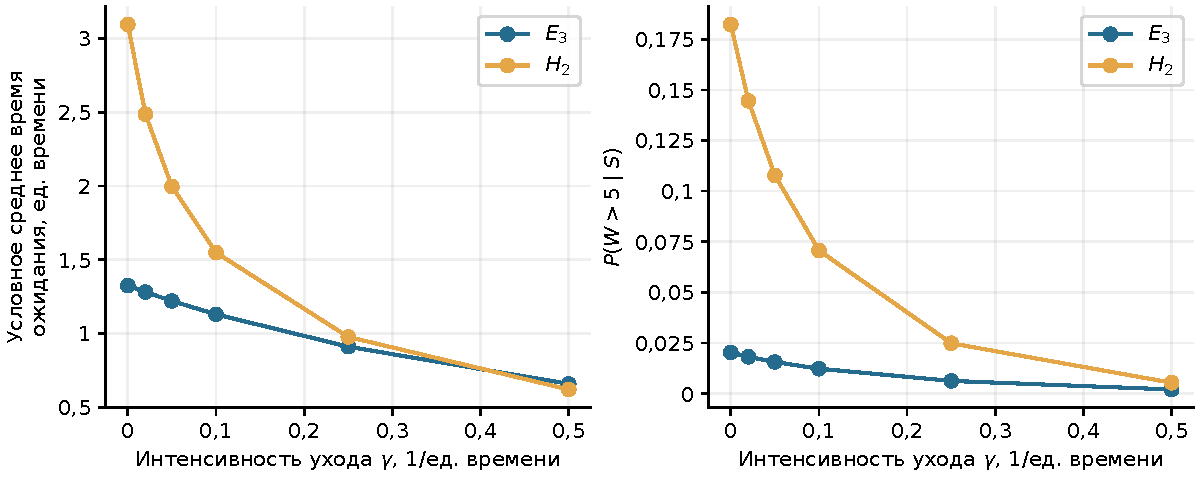
\includegraphics[width=\linewidth]{../figures/revision_conditional.pdf}
\caption{Среднее время ожидания и вероятность превышения срока при условии начала обслуживания: $D=5$, $\lambda=0{,}8$, $a=2$, $b=8$.}\label{fig:conditional}
\end{figure}

Порог запуска определяет соотношение времени накопления пакета и ожидания освобождения канала. На рисунке~\ref{fig:threshold} показана зависимость среднего ожидания от порога при разных нагрузках и законах обслуживания, на рисунке~\ref{fig:tails} --- значения ДФР для выбора максимального размера пакета. Выбор проводится по ДФР при заданном сроке $D$. Сопоставление ограничено исследованными сроками и не использует хвостовую асимптотику; различия вероятностей менее $10^{-7}$ считаются численно неразличимыми.

\begin{figure}[htbp]\centering
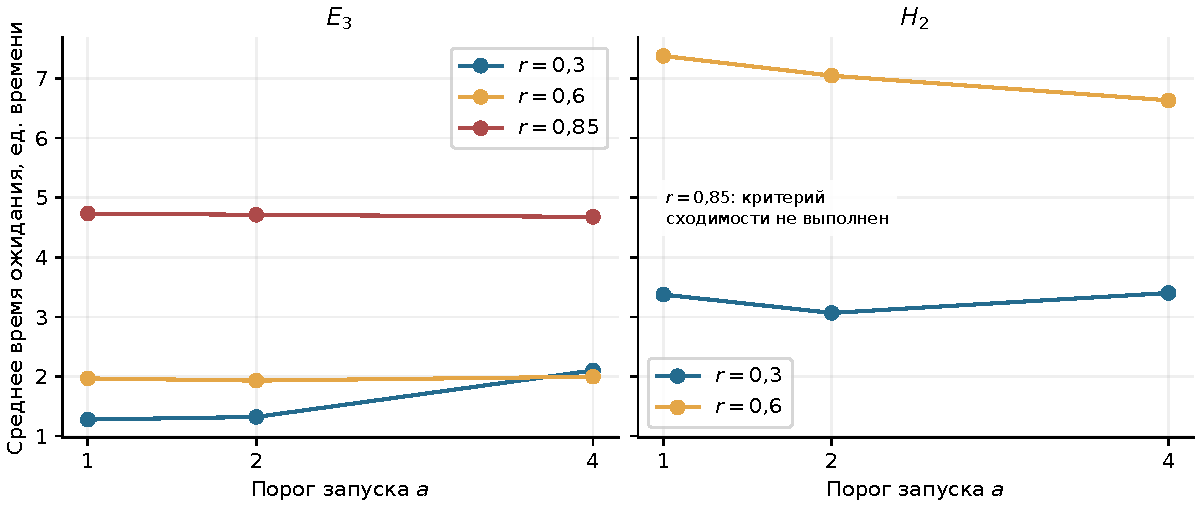
\includegraphics[width=\linewidth]{../figures/revision_threshold.pdf}
\caption{Среднее время ожидания при $b=8$, $\gamma=0$ и характеристике нагрузки $r=\lambda g(8)/8$. Для $H_2$ при $r=0{,}85$ критерий численной сходимости не выполнен.}\label{fig:threshold}
\end{figure}

\begin{figure}[htbp]\centering
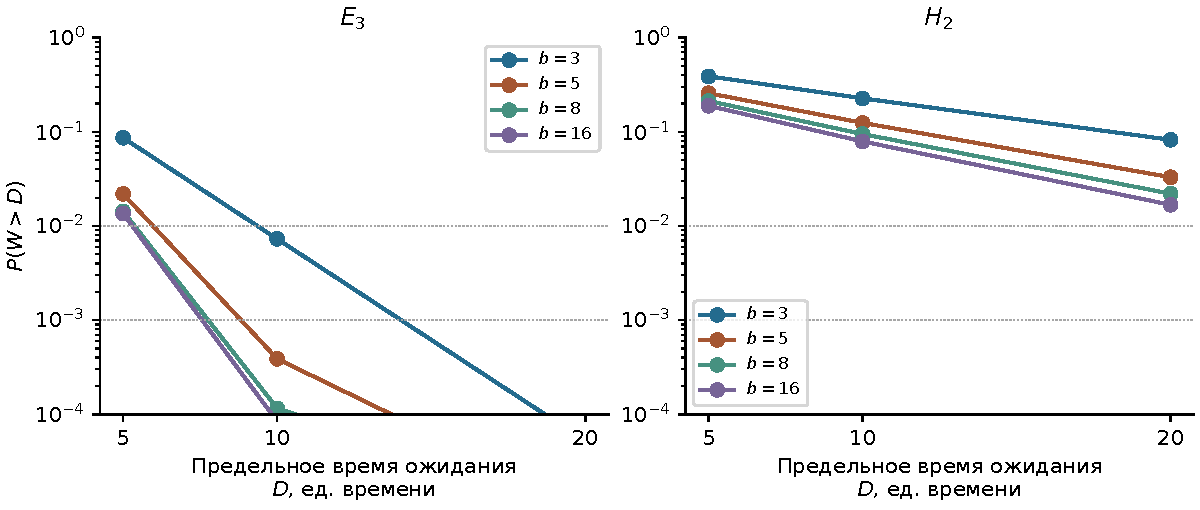
\includegraphics[width=\linewidth]{../figures/revision_tails.pdf}
\caption{Дополнительная функция распределения времени ожидания при $a=1$, $\gamma=0$, $\lambda=0{,}8$. Пунктиром обозначены уровни $10^{-2},10^{-3},10^{-4}$. Значения за нижней границей рисунка не следует считать нулевыми.}\label{fig:tails}
\end{figure}

\section*{Д. Аппроксимации и полный набор примеров выбора}

Сравним два приближения условного распределения времени ожидания. В первом параметры гамма-распределения определяются по первым двум начальным моментам $m_1,m_2$ времени $W$ при условии $S$. Во втором сохраняется вероятность нулевого ожидания $z=P(W=0\mid S)$, а положительная часть распределения аппроксимируется гамма-распределением по моментам $m_n/(1-z)$; соответствующая ДФР равна $(1-z)\overline G(D)$. В таблицах эти приближения обозначены как «Гамма» и «Атом + гамма». Оба построены по одним и тем же рассчитанным моментам. Для безусловного критерия используется величина $1-p_S[1-\widehat{\overline F}_S(D)]$, где $\widehat{\overline F}_S$ --- выбранная аппроксимация, а $p_S$ сохраняет значение, рассчитанное по марковской модели. Сопоставление тем самым выделяет влияние формы аппроксимации при заданных моментах и вероятности начала обслуживания.

Для условного критерия приняты допустимые значения $\varepsilon=10^{-2},10^{-3},10^{-4}$, для безусловного --- $0{,}1;0{,}05;0{,}01$. Каждый критерий и каждое приближение проверены в 2052 сочетаниях параметров системы, срока и допуска. Ошибочным признанием допустимости назовём случай, когда по приближению требование выполнено, а по расчёту марковской модели --- нет. Ошибочное отклонение означает обратное несоответствие. Если хотя бы одно из сравниваемых значений отличается от порога не более чем на $10^{-7}$, решения считаются неразличимыми в пределах принятого численного допуска. Таких случаев в рассмотренной серии нет. Итоги приведены в основном тексте статьи.

В таблице~\ref{tab:caps} приведены минимальные допустимые размеры пакета для всех девяти сочетаний срока и допуска при указанных параметрах.

\begin{table}[htbp]\centering\small
\caption{Наименьшее значение $b\in\{2,\ldots,16\}$, удовлетворяющее условию $\overline F_S(D)\leq\varepsilon$, при $E_3$-обслуживании, $a=1$, $\lambda=0{,}8$, $\gamma=0$. Прочерк --- отсутствие допустимого значения в этом диапазоне}\label{tab:caps}
\begin{tabular}{rrrrr}
\hline
$D$ & $\varepsilon$ & Расчёт & Гамма & Атом + гамма \\
\hline
5 & 0,01 & --- & --- & --- \\
5 & 0,001 & --- & --- & --- \\
5 & 0,0001 & --- & --- & --- \\
10 & 0,01 & 3 & 3 & 3 \\
10 & 0,001 & 5 & 5 & 4 \\
10 & 0,0001 & 10 & --- & --- \\
20 & 0,01 & 3 & 3 & 3 \\
20 & 0,001 & 3 & 3 & 3 \\
20 & 0,0001 & 3 & 3 & 3 \\
\hline
\end{tabular}

\end{table}

\section*{Е. Сопоставление с моделью Inoue}

Влияние ограничения размера пакета можно выделить, сохранив детерминированное время обслуживания $g(i)$ и сопоставив конечные $b$ с моделью Inoue~\cite{inoue2021}. В этой работе получена оценка сверху среднего полного времени пребывания при неограниченном размере пакета (теорема~2); обозначенному там времени $W$ здесь соответствует $V$. Рассмотрены 10 вариантов: $a=1$, $\gamma=0$, $\lambda=0{,}2;0{,}8$, $b=4,8,16,32,\infty$. При конечных $b$ использовано ИМ, а при $b=\infty$ --- также расчёт по вложенной цепи Маркова. Это отдельное сопоставление по среднему времени пребывания при одинаковом законе обслуживания, а не приближение ДФР для $E_k$ или $H_2$.

\begin{table}[htbp]\centering\small
\caption{Среднее время пребывания при детерминированном обслуживании $g(i)$, $a=1$, $\gamma=0$: ИМ, расчёт по вложенной цепи и оценка сверху}\label{tab:inoue}
\begin{tabular}{rrrrr}
\hline
$\lambda$ & $b$ & ИМ: $E[V]$, 95\% ДИ & $E[V]$, расчёт & Оценка сверху \\
\hline
0,2 & 4 & [2,4404; 2,4428] & --- & --- \\
0,2 & 8 & [2,4403; 2,4427] & --- & --- \\
0,2 & $\infty$ & [2,4403; 2,4427] & 2,4422 & 2,4679 \\
0,8 & 4 & [3,2953; 3,2998] & --- & --- \\
0,8 & 8 & [3,2392; 3,2425] & --- & --- \\
0,8 & $\infty$ & [3,2391; 3,2424] & 3,2430 & 3,3532 \\
\hline
\end{tabular}

\end{table}

При $\lambda=0{,}2$ интервальные оценки среднего времени пребывания для $b=4$, $b=8$ и $b=\infty$ перекрываются. При $\lambda=0{,}8$ ограничение $b=4$ увеличивает среднее время пребывания: соответствующий ДИ целиком лежит выше интервалов для $b=8$ и $b=\infty$, которые перекрываются (таблица~\ref{tab:inoue}). Следовательно, в рассматриваемом примере влияние ограничения размера пакета зависит от интенсивности входящего потока.

При $b=\infty$ расчёт по вложенной цепи даёт среднее время пребывания $2{,}442181$ для $\lambda=0{,}2$ и $3{,}243011$ для $\lambda=0{,}8$; соответствующие оценки сверху равны $2{,}467870$ и $3{,}353239$. Во втором случае расчёт находится вне ДИ $[3{,}239147;3{,}242448]$, полученного по ИМ. Результаты относятся к двум указанным интенсивностям; применение модели с неограниченным пакетом к системе с заданным конечным $b$ требует отдельного сопоставления.

\section*{Ж. Близкие модели в литературе}

Таблица~\ref{tab:prior} сопоставляет постановки и рассматриваемые характеристики. Она дополняет краткий обзор основного текста; перечисленные результаты не переносятся на модель с нетерпением без проверки условий.

\begin{table}[htbp]
\centering\small
\caption{Известные результаты по близким моделям пакетного обслуживания}\label{tab:prior}
\begin{tabular}{p{.22\linewidth}p{.36\linewidth}p{.34\linewidth}}
\hline
Работа & Рассмотренный результат & Существенное отличие \\\hline
Medhi~\cite{medhi1975} & Стационарное распределение времени ожидания и его моменты при правиле $(a,b)$ & Простейший поток, экспоненциальное обслуживание; нетерпение не учитывается \\
Banerjee и др.~\cite{banerjee2015} & Совместные стационарные распределения при марковском входящем потоке и зависимости обслуживания от размера пакета & Ограниченная вместимость очереди; более общий входящий поток \\
Claeys и др.~\cite{claeys2013} & Аппроксимация дополнительной функции распределения времени ожидания по полюсам и вычетам & Дискретное время, групповой входящий поток, ограничение времени накопления \\
van Ommeren и др.~\cite{vanommer2020} & Фазовое представление времени ожидания с учётом числа заявок перед помеченной и позади неё & Неоднородные каналы; интенсивность обслуживания не зависит от размера пакета; нетерпение не учитывается \\
Chaudhry и др.~\cite{chaudhry2023} & Расчёт распределения длины очереди методом корней и распределения времени ожидания с аппроксимацией Паде & Ограниченная вместимость очереди, одинаковый закон обслуживания пакетов \\
\hline
\end{tabular}
\end{table}
